\cotefile{11}
\scanpage{43}
\mspage{-3.7-}
% archive sheet number: 42
(identifying $\handwritten{\mathbb{A}}_R$ as $\handwritten{\mathbb{A}}^{n\unsure{\nu|v}-n}$), so that $(\handwritten{\mathbb{A}}^{n\nu-n},\handwritten{\phi}_R)$ is a geometric
quotient of $\handwritten{\unsure{\mathcal{U}|\mathscr{U}}}_R$ by $\mathrm{PGL}(n)$. Moreover, recall that
\[
\handwritten{\sigma}_R:\handwritten{\mathbb{A}}^{n\nu-n}\handwritten{\longrightarrow}\handwritten{\mathcal{U}}_R
\]
is a global section for $\handwritten{\phi}_R$. The following is obvious:

\uline{Corollary} \uline{3.2}: Suppose $\handwritten{\mathcal{U}\subset\mathcal{U}}_R$ is any invariant open subset. Then
$\handwritten{\mathcal{U}\cong}\mathrm{PGL}(n)\mathbin{\mathrm{x}}\handwritten{\sigma}_R^{-1}(\handwritten{\mathcal{U}})$, the isomorphism being compatible with the
obvious operations of $\mathrm{PGL}(n)$.

To illustrate these results, which may be somewhat obscured by the
cumbersome machinery of $R$-partitions, look at the case $\nu=1$, $S_1=\handwritten{\{}0,1,\ldots,n\handwritten{\}}$.
The proposition is then the classical result that $n+2$ points in
``general'' position in $\handwritten{\mathbb{P}}_n$ can be normalized to the canonical points
$(1,0,\ldots,0)$, $(0,1,\ldots,0),\ldots,(0,0,\ldots,1)$, and $(1,1,\ldots,1)$ by a unique
projective transformation. To give a second example, suppose $n=2$,
$\nu=2$,
\[
S_1=\handwritten{\{}0,1\handwritten{\}},\quad S_2=\handwritten{\{}1,2\handwritten{\}}.
\]
The proposition asserts that, given 5 points $P_0,P_1,P_2,P_3$ and $P_4$ in
the plane, suppose $P_0,P_1$ and $P_2$ are not collinear, that $P_3$ is not
on the line $\overline{P_0P_2}$ or the line $\overline{P_1P_2}$ and that $P_4$ is not on the line
$\overline{P_0P_1}$ or $\overline{P_0P_2}$: then we can uniquely normalize $P_0,P_1,P_2$ to $(1,0,0)$,
$(0,L,0)$ and $(0,0,1)$ respectively, and normalize $P_3$ to $(1,1,a)$, $P_4$
to $(b,1,1)$ by a suitable projective transformation. (cf. \handwritten{Figure 3},
where $Q_3=(1,1,0)$, $Q_4=(0,1,1)$ ).

\scanpage{44}
% archive sheet number: 43
Variantes évidentes avec des variétés topologiques compactes.
On peut prendre pour $h$ un anneau \inserted{(\unsure{ou corps|bien sûr|par exemple})}, lorsqu'on a une théorie
de cohomologie à coefficients dans $h$ \deleted{\unsure{qui satisfait}} \inserted{telle que}
\deleted{\unsure{Poincaré}} $H^*(X)$ satisfait à Poincaré \deleted{\illegible{1}} (pas seulement
mod torsion \ldots).

2) Considérons un autre foncteur de $V$ en les
anneaux bivariants jaugés, tels le foncteur
$A^*(X)$ (anneau de Chow, \deleted{\unsure{augmenté|gradué}} jaugé par le
\uline{degré} des \deleted{\unsure{co|0-}}cycles de degré max), ou un foncteur
quotient (tel les groupes de cycles mod équival.
numérique, homologique, \inserted{$\tau$,} algébriques, Picard, Albanese \ldots).
On trouve un anneau bivariant jaugé simplicial, qui
n'a plus aucune tendance à être spécial, et dont
les composantes n'ont pas trop envie d'être de
Poincaré \ldots

On peut tensoriser par $\unsure{\mathbb{Q}|Q|\mathbf{Q}}$ \ldots

3) On peut prendre $K(X)$ [jaugé par $\chi$], considéré comme
gradué de degré 0 \ldots

\noindent\rule{.48\linewidth}{.3pt}

Formalisme des correspondances. Soit $C\in A(I\sqcup I')$. On
va lui associer une application
\[
x\mathrel{\unsure{\mapstochar\relbar|\mapsto|\longmapsto}} C(x)\ \text{ou}\ C.x\quad :\quad A(I)\longrightarrow A(I')
\]
Ce sera le composé (où $\alpha:I\mathrel{\unsure{-|\to}}I\sqcup I'$, $\alpha':I'\mathrel{-}I\sqcup I'$)
\diagram{\begin{tikzcd}[ampersand replacement=\&,column sep=small]
 A(I)\arrow[r,"{\deleted{\leftarrow}\alpha^*}"] \& A(I\sqcup I')\arrow[r,"{y\mapsto Cy}"] \& A(I\sqcup I')\arrow[r,"{\alpha'_*}"] \& A(I')
\end{tikzcd}}
\margin{il y a un choix: prendre $Cy$ ou $yC$ !}

Ces actions sont connues quand on connaît, en plus
des lois d'\uline{anneaux} des $A(\unsure{+|*|\cdot})$, les $\alpha^*$ et $\alpha_*$
pour $\alpha:I\hookrightarrow J$ une injection [il suffit \unsure{mm|avec|même}
$\operatorname{card}(J)=\operatorname{card}(I)+1$, i.e $\alpha$ un ``opérateur face''].

\scanpage{45}
\mspage{-3.6-}
% archive sheet number: 44
for every $j\in\handwritten{\{}0,1,\ldots,n\handwritten{\}}$.

Note that $\handwritten{\lambda}_j$ is a section of $L_j\handwritten{\otimes}L_{\handwritten{\mu}(1)}^{-1}$ over the open set
$\handwritten{\unsure{\mathcal{U}|\mathscr{U}}}_R$. We now define
\[
\handwritten{\phi}:\handwritten{\mathcal{U}}_R\handwritten{\longrightarrow}\mathrm{PGL}(n)\mathbin{\mathrm{x}}\handwritten{\mathbb{A}}_R
\]
by its two components $p_1\circ\handwritten{\phi}$ and $p_2\circ\handwritten{\phi}$. The projective group
$\mathrm{PGL}(n)$, is, by definition,the affine open subset of
\[
\handwritten{\mathbb{P}}_{n^2+2n}=\operatorname{Proj}\handwritten{\mathbb{Z}}[a_{00},\ldots,a_{0n};\ a_{10},\ldots,a_{1n};\ \ldots;\ a_{n0},\ldots,a_{nn}]
\]
where $\det(a_{ij})\ne 0$. Therefore $p_1\circ\handwritten{\phi}$ is determined by
\[
\begin{aligned}
(p_1\circ\handwritten{\phi})^*(\underline{o}_{\handwritten{\mathbb{P}}}(1))&=L_{\handwritten{\mu}(1)}\\
(p_1\circ\handwritten{\phi})^*(a_{ij})&=X_i^{(j)}\handwritten{\otimes}(-1)^j\handwritten{\lambda}_j^{-1}.
\end{aligned}
\]
Finally the morphism $p_2\circ\handwritten{\phi}$ into affine space is determined by:
\[
(p_2\circ\handwritten{\psi})^*\left(x_i^{(n+k)}\right)=
\frac{D_{0,1,\ldots,\handwritten{\hat{i}},\ldots,n,n+k}}{D_{0,1,\ldots,\handwritten{\widehat{\mu(k)}},..,n,n+k}}\mathbin{\unsure{\cdot|\circ}}
\frac{\handwritten{\lambda}_i}{\handwritten{\lambda}_{\handwritten{\mu}(k)}}
\]
(It should be noted that the expression on the right is actually a
section of $\underline{o}_{\handwritten{\mathbb{A}_R}}$ ). Modulo the mechanical verifications that remain,
this proves the Proposition. \quad\uline{QED}

Of the morphisms constructed in the course of the above proof, it
is useful to \deleted{\unsure{set}} \handwritten{fix the notation}:
\[
\handwritten{\phi}_R=p_2\circ\handwritten{\phi}:\handwritten{\mathcal{U}}_R\handwritten{\longrightarrow}\handwritten{\mathbb{A}}^{n\unsure{\nu|v}-n}
\]

\scanpage{46}
% archive sheet number: 45
Posons $A(I',I)$ au lieu de $A(I\sqcup I')$. \inserted{\deleted{\unsure{(A corr.|Corresp.}} ($A$ des \deleted{\unsure{de|des}} \unsure{corr.|corresp.} de $I:I'$)}
On a à définir une application naturelle $h$-bilinéaire
\[
 A(I'',I')\times A(I',I)\longmapsto A(I'',I)
\]
notée \qquad $(v,u)\longmapsto v\circ u$, \qquad et définie par
\[
 v\circ u=p_{31*}\bigl(p_{21}^*(u)\,p_{32}^*(v)\bigr)
\]
\diagram{\begin{tikzcd}[ampersand replacement=\&,row sep=small,column sep=small]
 \& X^{I\sqcup I'}\arrow[dl,"\alpha"']\arrow[dr,"\alpha'"] \& \\
 X^I \& \& X^{I'}
\end{tikzcd}}
Ceci posé, si $\widetilde u:A(I)\mathrel{\unsure{-|\to}} A(I')$, \deleted{\unsure{et $\widetilde v$}} \ldots{} on
vérifie la formule
\[
 \widetilde{v\circ u}=\widetilde v\circ\widetilde u
\]
\diagram{\begin{tikzcd}[ampersand replacement=\&,row sep=small,column sep=small]
 \&\&\&X^{I\sqcup I'\sqcup I''}\arrow[dll,"p_{21}"']\arrow[dd,"p_{31}"]\arrow[drr,"p_{32}"]\&\&\&\\
 \&X^{I\sqcup I'}\arrow[dl,"\gamma"']\arrow[dr,"\gamma'"]\&\&\&\&X^{I'\sqcup I''}\arrow[dl,"\alpha'"']\arrow[dr,"\alpha''"]\&\\
 X^I\&\&X^{I'}\&X^{I\sqcup I''}\arrow[dl,no head,"\beta"']\arrow[dr,no head,"\beta''"]\&X^{I'}\&\&X^{I''}\\
 \&\&X^I\&\&X^{I''}\&\&
\end{tikzcd}}
En effet, on a
\[
\begin{aligned}
\widetilde{(v\circ u)}(x)&\overset{\text{def de }\widetilde{\deleted{\unsure{u}}}}{=}
 \deleted{\unsure{\beta^*(x)}}\beta''_*\bigl[(v\circ u)\,\beta^*(x)\bigr]\\
&\overset{\text{def de }v\circ u}{=}\beta''_*\bigl[
 \underbrace{p_{31*}\bigl(p_{21}^*(u)\,p_{32}^*(v)\bigr)\,\beta^*(\unsure{u|x})}_{\parallel\ \text{form. de proj}}\bigr]\\
&=p_{31*}\bigl(p_{21}^*(u)\,p_{32}^*(v)\,
 \underbrace{p_{31}^*\beta^*(x)}_{p_1^*(x)}\bigr)\\
&\overset{\text{transitivité}}{=}p_{3*}\bigl(p_{21}^*(u)\,p_{32}^*(v)\,p_1^*(x)\bigr)\\
&\deleted{\overset{\text{projection}}{=}p_{3*}\bigl(p_{21}^*(u)\,p_{32}^*(v)\bigr)x}
\end{aligned}
\]
\[
\begin{aligned}
\widetilde v(\widetilde u(x))&\overset{\text{def }\widetilde v}{=}
\deleted{\unsure{\alpha^*(\widetilde u(x))}}\alpha''_*\bigl(v\,\alpha'^*(\widetilde u(x))\bigr)\\
&\overset{\text{def }\widetilde u}{=}\alpha''_*\bigl(v\,
 \underbrace{\alpha'^*\bigl(\gamma'_*(u\,\gamma^*(x))\bigr)}_{\deleted{\unsure{p_*(x)x}}\ \parallel\ \text{échange}}\bigr)\ \deleted{=}\\
&\hspace{1em}\deleted{\unsure{p}}p_{32*}\bigl(p_{21}^{\unsure{+*|*}}(u\,\gamma^*(x))\bigr)
=p_{32*}\bigl(p_{21}^*(u)\,\underbrace{p_{21}^*\gamma^*(x)}_{p_1^*(x)}\bigr)
\end{aligned}
\]
\margin{``axiome cartésien'' oublié !}
\diagram{\begin{tikzcd}[ampersand replacement=\&,row sep=small,column sep=small]
 \&X^{I\sqcup I'\sqcup\deleted{\unsure{X}}I''}\arrow[dl,"p_{21}"']\arrow[dr,"p_{32}"]\&\&\\
 X^{I\sqcup I'}\arrow[dr,"\gamma'"']\&\&X^{I'\sqcup I''}\arrow[dl,"\alpha'"]\arrow[dr,no head,"\alpha''"]\&\\
 \&X^{I'}\&\&X^{I''}
\end{tikzcd}}
\[
\begin{aligned}
&=\alpha''_*\bigl(\underbrace{v\,p_{32*}(p_{21}^*(u)\,p_1^*(x))}_{\parallel\ \text{formule de projection, \uline{mod signe}}}\bigr)=\\
&\deleted{\unsure{=\alpha}}\quad\underbrace{\alpha''_*p_{32*}}
 \bigl(p_{32}^*(v)\,p_{21}^*(u)\,p_1^*(x)\bigr)\\
&\hspace{3em}p_{3*}\bigl(\overset{\scriptscriptstyle\parallel}{p}_{32}^*(v)\,p_{21}^*(u)\,p_1^*(x)\bigr)
\end{aligned}
\]
\margin{OK mod \uline{signe}, à faire \uline{attention}}

\scanpage{47}
\mspage{-3.4-}
% archive sheet number: 46
space. Then there is a $\mathrm{PGL}(n)$-linear isomorphism:
\begingroup\makeatletter\tagsleft@true\makeatother
\[
\handwritten{\unsure{\mathcal{U}|\mathscr{U}}}_R\handwritten{\cong}\mathrm{PGL}(n)\mathbin{\mathrm{x}}
\handwritten{\mathbb{A}}^{n\unsure{\nu|v}-n}\tag*{(*)}
\]
\endgroup
Hence $\handwritten{\mathcal{U}}_R$ is a globally trivial principal fibre bundle with respect
to the action of $\mathrm{PGL}(n)$, with base space $\handwritten{\mathbb{A}}^{n\nu-n}$.

\uline{Proof}: We shall construct morphisms from the left hand side of
$(*)$ to the right, and vice versa, leaving it to the reader to check
that they are mutually inverse. The morphisms will be obviously $\mathrm{PGL}(n)$-linear. First of all, we identify $\handwritten{\mathbb{A}}^{n\nu-n}$ with the scheme:
\[
\handwritten{\mathbb{A}}_R=\operatorname{Spec}
\frac{\handwritten{\mathbb{Z}}\bigl[x_0^{(n+1)},\ldots,x_n^{(n+1)};\ x_0^{(n+2)},\ldots,x_n^{(n+2)};\ldots;\ x_0^{(n+\nu)},\ldots,x_n^{(n+\nu)}\bigr]}
{\text{Ideal generated by }\handwritten{\{}x_i^{(n+k)}-1\mathrel{\big|}i\in S_k\handwritten{\}}}
\]
since both are affine spaces of dimension $n\nu-n$. Then a morphism
\[
\unsure{S|s}_R:\handwritten{\mathbb{A}}_R\handwritten{\longrightarrow}\handwritten{\mathcal{U}}_R
\]
is defined by the collection of composite morphisms
\[
S_i:\handwritten{\mathbb{A}}_R\handwritten{\xrightarrow{S}}\handwritten{\mathcal{U}}_R\handwritten{\subset}
(\handwritten{\mathbb{P}}_n)^{n+\nu+1}\handwritten{\xrightarrow{p_i}}\handwritten{\mathbb{P}}_n
\]
and $S_i$ is defined by the conditions (cf. EGA 2, \handwritten{4.2.3} ):
\[
\begin{aligned}
 S_i^*(\underline{o}\,(1))&\handwritten{\cong}\underline{o}_{\handwritten{\mathbb{A}}}\\
 S_i^*(X_j)&=\handwritten{\delta}_{ij}\quad\text{if }\ 0\leq i\leq n\\
 S_i^*(X_j)&=x_j^{(i)}\quad\text{if }\ n+1\leq i\leq m
\end{aligned}
\]

\scanpage{48}
% archive sheet number: 47
On va définir aussi
\[
 \deleted{\unsure{\delta}}\Delta_I\in A(I\sqcup I)
\]
qui \unsure{ser.|sera} tel que
\[
 \widetilde{\delta}_I(x)=x\qquad (x\in A(I))\qquad \text{i.e.}\quad \widetilde{\delta}_I=\mathrm{id}_{A(I)}.
\]
Pour \deleted{\unsure{$\delta$}} le voir, on \deleted{définit} considère $\delta:I\sqcup I\mathrel{\unsure{-|\to}}I$
d'où $\delta^{\deleted{*}}_*:A(I)\mathrel{-}A(I\sqcup I)$, on pose
\[
 \Delta_I=\delta_*(1)
\]
On aura (\deleted{\unsure{écrivant}} $\Delta$ au lieu de $\Delta_I$
\diagram{\begin{tikzcd}[ampersand replacement=\&,column sep=small,row sep=small]
 \&X^I\arrow[d,"\delta"]\&\\
 \&X^{I\sqcup I}\arrow[dl,"p_1"']\arrow[dr,"p_2"]\&\\
 X^I\&\&X^I
\end{tikzcd}}
\[
\begin{aligned}
 \widetilde{\deleted{\unsure{\delta}}\Delta}(x)&\overset{\text{déf de }\sim}{=}p_{2*}\bigl(\Delta\,p_1^*(x)\bigr)\\
 &=p_{2*}\bigl(\underbrace{\delta_*(1)\,p_1^*(x)}_{\parallel}\bigr)\\
 &\hspace{4em}\deleted{\unsure{p_1|p}}\delta_*\bigl(\unsure{\Gamma|\delta}^*p_1^*(x)\bigr)=\delta_*(x)\\
 &=p_{2*}\,\delta_*(x)=x
\end{aligned}
\]
Il faut encore définir l'associativité de
l'opération $\circ$, et le fait que les $\delta_I$ jouent le
rôle d'unités. On voit que sous ces conditions,

\scanpage{49}
\mspage{-3.3-}
% archive sheet number: 48
$0\leq\handwritten{\alpha}_i\leq m$, let
\[
 D_{\handwritten{\alpha_0,\ldots,\alpha_n}}=\underset{\handwritten{0\leq i,j\leq n}}{\det}
 \handwritten{\bigl[}X_i^{\handwritten{(\alpha_j)}}\handwritten{\bigr]}
\]
be the section of $L_{\handwritten{\alpha_0}}\handwritten{\otimes}\cdots\handwritten{\otimes}L_{\handwritten{\alpha_n}}$ obtained by addition and tensor
product as in the determinant. It is evident that $D_{\handwritten{\alpha_0,\ldots,\alpha_n}}$ is an
\uline{invariant} section of $L_{\handwritten{\alpha_0}}\handwritten{\otimes}\cdots\handwritten{\otimes}L_{\handwritten{\alpha_n}}$. The non-vanishing of suitable
$D$'s defines the open sets we are looking for.

\uline{Definition} \uline{3.2}: An \uline{$R$}-\uline{partition} of $\handwritten{\{}0,1,\ldots,n\handwritten{\}}$ is an ordered set
of subsets $S_1$, $S_2$, $\ldots$, $S_{\unsure{\nu|v}}$ of $\handwritten{\{}0,1,\ldots,n\handwritten{\}}$ such that

(i) $S_i\handwritten{\cap}(S_{i-1}\handwritten{\cup}\cdots\handwritten{\cup}S_2\handwritten{\cup}S_1)$ consists of exactly one
integer, for $2\leq i\leq\nu$,

(ii) $\displaystyle\handwritten{\bigcup_{i=1}^{\nu}}S_i=\handwritten{\{}0,1,\ldots,n\handwritten{\}}$,

\uline{Definition} \uline{3.3}: Given an $R$-partition $R=\handwritten{\{}S_1,\ldots,S_\nu\handwritten{\}}$, let
$\handwritten{\unsure{\mathcal{U}|\mathscr{U}}}_R\handwritten{\subset}(\handwritten{\mathbb{P}}_n)^{n+\nu+1}$ be the open subset defined by

(i) $D_{0,1,\ldots,n}\ne 0$,

(ii) for all $k$ between 1 and $\nu$, and for all $i\in S_k$
\[
 D_{0,1,..\handwritten{\hat{i}},..,n,n+k}\ne 0
\]
Not only is $\handwritten{\mathcal{U}}_R$ affine, but the whole structure of the action
of $\mathrm{PGL}(n)$ on $\handwritten{\mathcal{U}}_R$ can be described explicitly:

\uline{Proposition} \uline{3.1}: Let $R=\handwritten{\{}S_1,\ldots,S_\nu\handwritten{\}}$ be an $R$-partition of
$\handwritten{\{}0,1,\ldots,n\handwritten{\}}$. Let $\mathrm{PGL}(n)$ act on $\mathrm{PGL}(n)\mathbin{\mathrm{x}}\handwritten{\mathbb{A}}^{n\nu-n}$ by the product
of left translation on itself and the trivial action on the affine

\scanpage{51}
% archive sheet number: 50
\unsure{Sous-algèbre|Sous-algèbres} \unsure{tautologique|tautologiques} \unsure{des|de} $H^*(X^n)$.

\textcircled{1} \uline{$H^*(X)$}\qquad\deleted{degrés}

\diagram{$\begin{array}{lll}
 \text{\uline{générateurs}} & y\in H^{\unsure{n|m}}(X) &\\
 \text{\uline{relation}s} & y^2=0 &\\
 \text{\uline{base}} & \text{deg. }0 &1\\
 &\text{deg. }n &y
\end{array}$}

\textcircled{2} \uline{$H^*(X\times X)$}

\uline{générateurs}:\qquad $y\otimes1=y_1$ \deleted{\unsure{1}}, $1\otimes y=y_2$, $\delta\qquad\in H^n(X)$

\uline{relations}\qquad $y_1^2=y_2^2=0$, $y_1y_2=y_1\delta=y_2\delta$; $\delta^2=\chi\,y_1y_2$\qquad
($\chi\in\mathbb{Z}$ la \unsure{car|car.} d'EP)

\diagram{$\begin{array}{lll}
 \text{\uline{base}} & \text{deg }0 &1\\
 &\text{deg }n &y_1,y_2,\delta\\
 &\text{deg }2n &y_1y_2y_3
\end{array}$}

\textcircled{3} $H^*(X\times X\times X)$

\diagram{$\begin{array}{lll}
 \text{\uline{générateurs}} & \text{degr }n:\ \cdot &
 y\otimes1\otimes1=y_1,\quad 1\otimes y\otimes1=y_2,\quad 1\otimes1\otimes y=y_3,\quad
 \delta_{12}=\delta\otimes1,\delta_{23},\delta_{31}\\
 &\text{deg }2n &\delta
\end{array}$}

\uline{relations}
\[
\left\{\begin{aligned}
 &y_1^2=y_2^2=y_3^2=0\\
 &\delta_{12}^2=\chi\,y_1y_2,\ \delta_{23}^2=\chi\,y_2y_3,\ \delta_{31}^2=\chi\,y_3y_1,\ 
 \delta_{12}\delta_{23}=\delta_{12}\delta_{31}=\delta_{23}\delta_{31}=\delta\\
 &\delta_{12}y_1=\delta_{12}y_2=\deleted{\unsure{\delta}}y_1y_2,\ 
 \delta_{23}y_2=\delta_{23}y_3=y_2y_3,\ \delta_{31}y_3=\delta_{31}y_1=y_3y_1\\
 &\delta y_1=\delta y_2=\delta y_3=y_1y_2y_3\\
 &\delta^2=0\\
 &\delta_{12}\delta=\delta_{23}\delta=\delta_{31}\delta=\chi\,y_1y_2y_3
\end{aligned}\right.
\]
\diagram{$\begin{array}{lll}
 \text{\uline{base}} &\text{deg }0&1\\
 &\text{deg }n&y_1,y_2,y_3,\delta_{12},\delta_{23},\delta_{31}\\
 &\text{deg }2n&y_1y_2,y_2y_3,y_3y_1,\delta_{12}y_3,\delta_{23}y_1,\delta_{31}y_2,\delta\\
 &\text{deg }3n&y_1y_2y_3
\end{array}$}

\figure{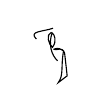
\begin{tikzpicture}[x=0.23cm,y=0.23cm]
 \draw[thin] (0,2.7) .. controls (-.45,3.15) and (.35,3.1) .. (.92,3.3);
 \draw (.83,3.08) .. controls (.51,2.95) and (.67,2.40) .. (.89,2.25)
 .. controls (1.16,2.6) and (.98,2.99) .. (.87,3.04)
 .. controls (.65,2.43) and (.83,1.81) .. (1.17,1.50);
 \draw (.94,2.14) .. controls (1.23,2.25) and (1.38,2.14) .. (1.5,2.05)
 .. controls (1.34,1.15) and (1.52,.72) .. (1.21,.30)
 -- (1.70,.67) -- (1.56,1.92)
 .. controls (1.43,2.35) and (1.1,2.02) .. (.94,2.14);
\end{tikzpicture}}

\scanpage{52}
\mspage{-3.18-}
% archive sheet number: 51
form $\handwritten{\unsure{\overline{\Phi}|\Phi}}_0^{-1}(V)$ for some open neighborhood $V$ of $y$. Since $\handwritten{\unsure{\mathcal{U}|\mathscr{U}}}_0$ is
affine, it follows (for example, by SGA 8, Cor. 5.6) that $V$ is
affine. Moreover, $\handwritten{\mathcal{U}}_0$ is defined by $P\ne 0$, where $P$ is an invariant section of $(L_0\handwritten{\otimes}\cdots\handwritten{\otimes}L_m)^N$ (for suitable $N$). Then $P^{n+1}$
is induced by a section $s$ of $(M_0\handwritten{\otimes}\cdots\handwritten{\otimes}M_m)^N$ (cf. \S1), and $V$
must be defined by $s\ne 0$. \quad\uline{QED}

For the sake of the sequel, we fix a \handwritten{more explicit} notation :
\handwritten{$(\mathbb{P}_n)^{m+1}_{\mathrm{stable}}$ instead of $\mathcal{U}_{\mathrm{stable}}$, (cf. Proposition 7.7)}.

\scanpage{53}
% archive sheet number: 52
\textcircled{$k$}\qquad $H^*(X^k)$\qquad\deleted{\uline{générateurs}}

\uline{générateurs}
\diagram{$\begin{array}{llll}
 \text{\uline{degré $n$}:}&\text{les }k\text{ transformés de}&
 y\otimes\underbrace{1\otimes ..\otimes1}_{k-1}&=\overline y\\
 &\text{les }\binom{k}{2}\text{ transformés de}&
 \delta_1^{\deleted{\unsure{1}}}\otimes\underbrace{1\otimes-\otimes1}_{k-2}&=\overline\delta_1\\
 \text{\uline{degré $2n$}:}&\text{les }\binom{k}{3}\text{ transformés de}&
 \delta_2\otimes\underbrace{1\otimes ..\otimes1}_{k-3}&=\overline\delta_2\\
 \cdots&&&\cdots\\
 \text{\uline{degré} }\unsure{k|r}n:&\text{les }\binom{k}{r+1}\text{ transformés de}&
 \delta_r\otimes\underbrace{1\otimes ..\otimes1}_{k-1-r}&=\overline\delta_r\\
 -\ \text{---}&\ddots&&\cdots\\
 \text{degré }(k-1)n:&\delta_{k-1}&&=\overline\delta_{k-1}
\end{array}$}

\deleted{\uline{relations}}

\uline{relations}

\scanpage{54}
\mspage{-3.17-}
% archive sheet number: 53
section of $\handwritten{\{}L_0\handwritten{\otimes}\cdots\handwritten{\otimes}L_m\handwritten{\}}^M$ for some $M$, and such that $\handwritten{\unsure{\mathcal{U}|\mathscr{U}}}_0\handwritten{\subset\mathcal{U}}_{\handwritten{\mathrm{stable}}}$.
\deleted{\unsure{stable.}}

\uline{Proof}: Let $N\geq N_0>0$, and $P_0,\ldots,P_m$ be given by the
Proposition. Moreover, let $P=P_0\handwritten{\otimes}\cdots\handwritten{\otimes}P_m$, and let $M=(m+1)N-N_0$.
Then $P$ is a section of the ample invertible sheaf $(L_0\handwritten{\otimes}\cdots\handwritten{\otimes}L_m)^M$;
hence $P\ne0$ defines an affine open neighborhood of $x$. Moreover,
if $P(y)\ne0$ for some geometric point $y$ of $(\handwritten{\mathbb{P}}_n)^{m+1}$, then
$P_0(y)\ne0,\ldots,P_m(y)\ne0$, hence $y$ is stable by Proposition 3.6.
\hfill\uline{QED}

We can now apply our work to obtain the final result. Let $(Z,\handwritten{\Phi})$
be the geometric quotient of $\handwritten{\mathcal{U}}_{\mathrm{reg}}$ by $\mathrm{PGL}(n)$. Let $Z_0\handwritten{\subset}Z$ be
the open subset such that $\handwritten{\Phi}^{-1}(Z_0)=\handwritten{\mathcal{U}}_{\mathrm{stable}}$. Let $\handwritten{\Phi}_0$ be the
restriction of $\handwritten{\Phi}$ to a morphism from $\handwritten{\mathcal{U}}_{\mathrm{stable}}$ to $Z_0$.

\uline{Theorem} \uline{3.8}: $(Z_0,\handwritten{\Phi}_0)$ is a geometric quotient of $\handwritten{\mathcal{U}}_{\mathrm{stable}}$ by
$\mathrm{PGL}(n)$, and, in fact, $\handwritten{\mathcal{U}}_{\mathrm{stable}}$ is a locally trivial principal
fibre bundle over $Z_0$ with group $\mathrm{PGL}(n)$. Moreover, $M_0\handwritten{\otimes}\cdots\handwritten{\otimes}M_m$
is ample on $Z_0$, hence $Z_0$ is a quasi-projective scheme.

\uline{Proof}: The first part is clear. To prove the second part, it
suffices to show that if $y$ is any geometric point of $Z_0$, then $y$
has an affine open neighborhood of the form $(Z_0)_s$ for some section
$s$ of $(M_0\handwritten{\otimes}\cdots\handwritten{\otimes}M_m)^N$, (cf. EGA 2, Remark following Theorem 4.5.2).
But let $x$ be a geometric point of $\handwritten{\mathcal{U}}_{\mathrm{stable}}$ over $y$. The open
neighborhood $\handwritten{\mathcal{U}}_0$ of Corollary 3.7 is invariant, hence of the

\scanpage{55}
% archive sheet number: 54
\diagram{\begin{tikzcd}[ampersand replacement=\&,row sep=small]
 X^{k-i}\arrow[r] \& X^k\\
 {} \& {[1,k']\subset[1,\unsure{k|h}]}\arrow[l,"\text{surj}"']
\end{tikzcd}}
\[
 X^I
\]
$I=I'\sqcup I''$\qquad $R$ relation d'équivalence sur $I'$

$I$ avec une division en \unsure{ens|un|un ens.} de parties \deleted{\unsure{non vides}}, comprenant la partie vide
et le choix d'une de ses parties
\[
 (R,J)\quad
 \left\{\begin{aligned}
 &R\subset\unsure{\mathcal P|\mathfrak P}(I)\text{ tel que }\deleted{\unsure{J}}
 \left\{\begin{aligned}
 &\text{a) }\bigsqcup_{J\in R}\deleted{\unsure{J}}A=I\\
 &\text{b) }\deleted{\unsure{J,J'}}A,A'\in R,\ \deleted{\unsure{J}}A\ne\deleted{\unsure{J'}}A'\Rightarrow
 \deleted{\unsure{J}}A\cap\deleted{\unsure{J'}}A'=\varnothing\\
 &\text{c) }\varnothing\in R\\
 &\deleted{\unsure{d}}
 \end{aligned}\right.\\
 &J\in R
 \end{aligned}\right.
\]
\[
 \varepsilon_{R,J}\,\varepsilon_{R',J'}=
 \left\{\begin{aligned}&0\quad\text{si }\ J\cap J'\ne\varnothing\\&\phantom{0}\end{aligned}\right.
\]
\deleted{\unsure{Si}} Supposons \qquad $J\cap J'=\varnothing$
\[
 Z_{R,J}=\left\{(x_i)_{i\in I}\quad\text{tels que }\left\{\begin{aligned}
 &x_i=\unsure{-|a}\quad\text{si }\ i\in J\\
 &x_i=x_j\quad\text{si }\ \exists A\in R,\ \text{tq. }\ i,j\in A
 \end{aligned}\right.\right\}
\]
\[
 Z_{R,J}^{a}\cap Z_{R',J'}^{a'}\underset{\text{du pt de vue ens.}}{=}Z_{R'',J''}
\]
$R''$ est la partition, \unsure{engendrée p.},
\uline{engendrée} par $R,R'$

$\widetilde J$ la classe \deleted{\unsure{de $J$}}\inserted{engendrée par} $J$

$\widetilde J'$ \deleted{\unsure{engendrée par}} $J'$

\[
 \deleted{\widetilde J\ne\widetilde J'}
\]
\[
\left|\begin{aligned}
 &\widetilde J=\widetilde J'\ne\varnothing\quad\Longrightarrow\quad\varepsilon_{R,J}\,\varepsilon_{R',J'}=0\\
 &\widetilde J\ne\widetilde J'\ \text{ou }\ \widetilde J=\widetilde J'=\varnothing\qquad\text{alors}\qquad
 \varepsilon_{R,J}\,\varepsilon_{R',J'}=
 \left(\prod_{i\in\widetilde J\cup\widetilde J'}\unsure{\eta|y}_i\right)
 \prod_{\substack{A''\in R''\\A''\ne\widetilde J\\A''\ne\widetilde J'}}
 \varepsilon^{\deleted{\unsure{A''}}}_{R_{\!A''}\deleted{\unsure{,J}}}
 \varepsilon^{\deleted{\unsure{A''}}}_{R'_{\!A''}\deleted{\unsure{,J'}}}
\end{aligned}\right.
\]
On est ramené au cas où $J=\varnothing,J'=\varnothing$,
et la relation d'équivalence \uline{engendrée} par $R,R'$ est la relation \uline{grossière}.

Alors, ensemblistement, on obtient la diagonale de $X^I$

\scanpage{56}
\mspage{-3.15-}
% archive sheet number: 55
suppose
\[
 \text{(i)}\qquad x^{(0)}=x^{(1)}=\cdots=x^{(\handwritten{\beta_0})}\ne x^{(\handwritten{\beta_0}+1)}
\]
(ii) $x^{(0)},x^{(1)},\ldots,x^{(\handwritten{\beta_1})}$ all lie on exactly one line, but
$x^{(\handwritten{\beta_1}+1)}$ is not on this line.

(iii) $x^{(0)},x^{(1)},\ldots,x^{(\handwritten{\beta_2})}$ all lie on exactly one plane, but
$x^{(\handwritten{\beta_2}+1)}$ is not in this plane,
\[
\substack{\cdot\\\cdot\\\cdot\\\cdot\\\cdot}
\]
(n) $x^{(0)},\ldots,x^{(\handwritten{\beta_{n-1}})}$ all lie in exactly one hyperplane, but
$x^{(\handwritten{\beta_{n-1}}+1)}$ is not in this hyperplane.

Then $x^{(0)},x^{(\handwritten{\beta_0}+1)},\ldots,x^{(\handwritten{\beta_{n-1}}+1)}$ do not lie in a hyperplane, hence
$D_{0,\handwritten{\beta_0}+1,\ldots,\handwritten{\beta_{n-1}}+1}(x)\ne0$; and whenever $D_{\handwritten{\alpha_0,\alpha_1,\ldots,\alpha_n}}(x)\ne0$, then
\[
 \handwritten{\alpha}_0\geq0,\quad\handwritten{\alpha}_1\geq\handwritten{\beta}_0+1,\quad
 \handwritten{\alpha}_2\geq\handwritten{\beta}_1+1,\ \ldots,\ \handwritten{\alpha}_n\geq\handwritten{\beta}_{n-1}+1.
\]
Therefore, the condition on $\handwritten{\ell}$ is that:
\begingroup\makeatletter\tagsleft@true\makeatother
\[
 \handwritten{\ell}\bigl(d_{0,\handwritten{\beta_0}+1,\ldots,\handwritten{\beta_{n-1}}+1}\bigr)\geq0.\tag*{(*)}
\]
\endgroup
But it is easy to check that the set of all $\handwritten{\{\lambda\}}$'s such that $\handwritten{\lambda}_0\leq\cdots\leq\handwritten{\lambda}_m$
and $\displaystyle\handwritten{\sum_{i=0}^{m}\lambda}_i=0$ is a convex set spanned by the particular set of
$\handwritten{\{\lambda\}}$'s given in the lemma. Therefore $(*)$ holds for some $\handwritten{\ell}$ if and only
if it holds for one of the extreme sets of $\handwritten{\{\lambda}_i\handwritten{\}}$. \quad\uline{QED}

Removing the assumption $\handwritten{\lambda}_0\leq\cdots\leq\handwritten{\lambda}_m$, and computing $\handwritten{\ell}$ we
conclude that the existence of the $P$'s is equivalent to:

\scanpage{57}
% archive sheet number: 56
\[
\begin{aligned}
 1\leq\operatorname{card}R=s\leq k&\qquad\text{donc}\quad\dim Z_R=\deleted{\unsure{k}}sn
   &\operatorname{codim} Z_R&=kn-sn=(k-s)n\\
 \operatorname{card}R'=s'&&\operatorname{codim} Z_{R'}&=(k-s')n\\
 \operatorname{card}R''=1&&\operatorname{codim} Z_{R''}&=(k-1)n
\end{aligned}
\]
\[
 (k-1)n\leq(k-s)n+(k-s')n\qquad\text{i.e.}\quad\deleted{\unsure{k\geq s+s'-1}}
\]
\[
 \boxed{s+s'\leq k+1}
\]
\margin{\uline{à vérifier}\quad\uline{OK}}
% slanted
Cas d'égalité \quad \uline{$s+s'=k+1$} : on trouve la diagonale $\delta_k$.

Cas d'inégalité \qquad $k+1>s+s'$\quad i.e. $k\deleted{\unsure{>}}\geq s+s'$
\[
 \left|\begin{aligned}
 &\deleted{\text{donc il faut }\text{\unsure{voir|avoir}}}\quad\deleted{\unsure{k\geq s+s'|k+1>s+s'}}\\
 &\text{1) }\ k>s+s'\quad\text{alors }\varepsilon_R\varepsilon_{R'}=0\quad\text{pour raison de degrés}\\
 &\text{2) }\ k=s+s',\quad\text{alors }\varepsilon_R\varepsilon_{R'}=\underset{?}{\chi}\,\unsure{\eta|y}_{X^k}
 \end{aligned}\right.
\]
\margin{\uline{à vérifier}}
% slanted
\diagram{\begin{tikzcd}[ampersand replacement=\&,column sep=small,row sep=small]
 X^s\arrow[r,hook] \& X^{\unsure{k|h}}\\
 \&X^{s'}\arrow[u,hook']
\end{tikzcd}}
$s+s'=k$ ou $k+1$

a) Stable par $\boxtimes$ : clair

b) Stable par image inverse par projection
simpliciale : clair \deleted{\unsure{simp}}

c) Stable par \unsure{image|images} \uline{\unsure{directe|directes}} par projection

\margin{\deleted{\unsure{$k\leq k-s+k-s'$}}}
\diagram{\begin{tikzcd}[ampersand replacement=\&,column sep=small,row sep=small]
 V^s\arrow[r]\&V^k\\
 V\arrow[u]\arrow[r]\&V^{s'}\arrow[u]
\end{tikzcd}}
$i\in I$ définit \unsure{quelles|quelle} projections
\[
 X^I\mathrel{\unsure{-|\to}} X^{I-\{i\}}
\]
a) $i\in J$ : clair

b) $i\notin J$ : on est ramené au cas de

\diagram{\begin{tikzcd}[ampersand replacement=\&,row sep=small,column sep=small]
 X^p\arrow[r]\&X^q\\
 X^p\times X\arrow[r,no head]\&X^q\times X\\
 \Delta_p\&\Delta_q\arrow[l,no head]\\
 \Delta_{p\sqcup1}\&\Delta_{q\sqcup1}\arrow[l]
\end{tikzcd}}
$\delta_I\in H^*(X^I)\longrightarrow H^*(X^{I-\{i\}})$

\deleted{\unsure{$X^I$}}\quad on trouve $\delta_I$

\deleted{d) \unsure{Relations|Relativement} \unsure{Stables par images} \unsure{que toutes les classes}
au delà des \unsure{opérations} des appl. simpliciales}

\diagram{\begin{tikzcd}[ampersand replacement=\&,row sep=small,column sep=small]
 \&U\arrow[dr,hook,no head,"p"]\&\\
 U\cap V\arrow[ur,hook,no head]\arrow[dr,hook,no head]\&\&W\\
 \&V\arrow[ur,hook,no head,"q"']\&
\end{tikzcd}}
$p+q-r$\qquad $r$

\diagram{\begin{tikzcd}[ampersand replacement=\&,row sep=small,column sep=small]
 \&U'\arrow[dr,no head,"p-r"]\&\&\\
 U'\cap V'\arrow[ur,no head,"{\deleted{p}q-r}"]\arrow[dr,no head,"p-r"']\&\&U'+V'\arrow[r,no head,"r"]\&W'\\
 \&V'\arrow[ur,no head,"q-r"']\&\&
\end{tikzcd}}
Stable par \unsure{cup|comp.}

\[
 \boxed{\text{engendré, via }\boxtimes,\ \text{par }\deleted{\unsure{\xi}},\eta,\text{ et les }\delta_I}
\]
\[
 (\delta_{\unsure{1|2}}\boxtimes\delta_2)
\]

\scanpage{58}
\mspage{-3.14-}
\[
\begin{aligned}
(1,\ldots,1)\mathrel{\handwritten{\in}}\text{interior of }C_x
&\mathrel{\handwritten{\Longleftrightarrow}}\text{ there are integers } N\geq N_0>0\\
&\phantom{\Longleftrightarrow}\text{ such that positive integral sums of}\\
&\phantom{\Longleftrightarrow}\text{ the }d\text{'s generating }C_x\text{ are}\\
&\phantom{\Longleftrightarrow}\text{ the points:}\\
&\phantom{\Longleftrightarrow}\ (N-N_0,N,\ldots,N),(N,N-N_0,\ldots,N),\\
&\phantom{\Longleftrightarrow}\ \ldots,(N,N,\ldots,N-N_0)\\[3pt]
&\mathrel{\handwritten{\Longleftrightarrow}}P_i,\text{ as in the Proposition, exist.}
\end{aligned}
\]
But on the other hand, $\handwritten{\{}(1,1,\ldots,1)\mathrel{\handwritten{\notin}}\text{ interior of }C_x\handwritten{\}}$ is equivalent to the existence of a linear functional $\handwritten{\ell}$ on $E$ such that $\handwritten{\ell\bigl(}(1,1,\ldots,1)\handwritten{\bigr)}=0$, and $\handwritten{\ell(}d_{\handwritten{\alpha_0,\ldots,\alpha_n}}\handwritten{)}\geq0$ for every $d$ generating $C_x$. Suppose
\[
\handwritten{\ell\bigl(}(Z_0,\ldots,Z_m)\handwritten{\bigr)}=\sum_{i=0}^{m}\handwritten{\lambda}_i Z_i\;.
\]
Without loss of generality, we may assume that $\handwritten{\lambda}_0\leq\handwritten{\lambda}_1\leq\ldots\leq\handwritten{\lambda}_m$. The key point is:

\uline{lemma}: If for some set of $\handwritten{\lambda}_i$ such that $\handwritten{\lambda}_0\leq\handwritten{\lambda}_1\leq\ldots\leq\handwritten{\lambda}_m$ and $\handwritten{\sum_{i=0}^{m}\lambda_i}=0$, then $\handwritten{\ell(}d_{\handwritten{\alpha_0,\ldots,\alpha_n}}\handwritten{)}\geq0$ for every $d_{\handwritten{\alpha_0,\ldots,\alpha_n}}$ generating $C_x$, then, in fact, this happens for some $\handwritten{\{\lambda_i\}}$ of the form:
\[
\begin{aligned}
&\handwritten{\lambda}_0=\handwritten{\lambda}_1=\ldots=\handwritten{\lambda_\beta}=-(m-\handwritten{\beta})\\
&\handwritten{\lambda_{\beta+1}}=\ldots=\handwritten{\lambda}_m=+(\handwritten{\beta}+1)\;.
\end{aligned}
\]
\uline{Proof}: The point is that if $\handwritten{\lambda}_0\leq\ldots\leq\handwritten{\lambda}_m$, then we can pick, \uline{a} \uline{priori}, that determinant $D_{\handwritten{\alpha_0,\ldots,\alpha_n}}$ which is not zero at $x$, and for which $\handwritten{\ell(}d_{\handwritten{\alpha_0,\ldots,\alpha_n}}\handwritten{)}=\handwritten{\sum_{i=0}^{n}\lambda_{\alpha_i}}$ assumes its minimum value. Namely,
% archive sheet number: 57

